%!TEX root = ../template.tex
%%%%%%%%%%%%%%%%%%%%%%%%%%%%%%%%%%%%%%%%%%%%%%%%%%%%%%%%%%%%%%%%%%%%
%% chapter5.tex
%% NOVA thesis document file
%%
%% Chapter with lots of dummy text
%%%%%%%%%%%%%%%%%%%%%%%%%%%%%%%%%%%%%%%%%%%%%%%%%%%%%%%%%%%%%%%%%%%%

\typeout{NT FILE chapter5.tex}%

\chapter{Simulation and Analysis}
\label{cha:simulations}

\epigraph{
	Whenever there is a problem, it usually lies between the chair and the monitor.
}{M. Xarepe}

Simulations are a fundamental component of modern nuclear physics experiments, providing a virtual environment where detector responses and physical processes can be modeled and tested prior to data acquisition. The work presented in this thesis was carried out using the R3BRoot framework, the dedicated simulation and analysis environment developed for experiments within the \gls{R3B} collaboration. Built upon the widely used Geant4 and ROOT packages, R3BRoot provides a comprehensive platform that combines accurate particle transport, flexible data handling, and experiment-specific detector models.

\begin{figure}
	\centering
	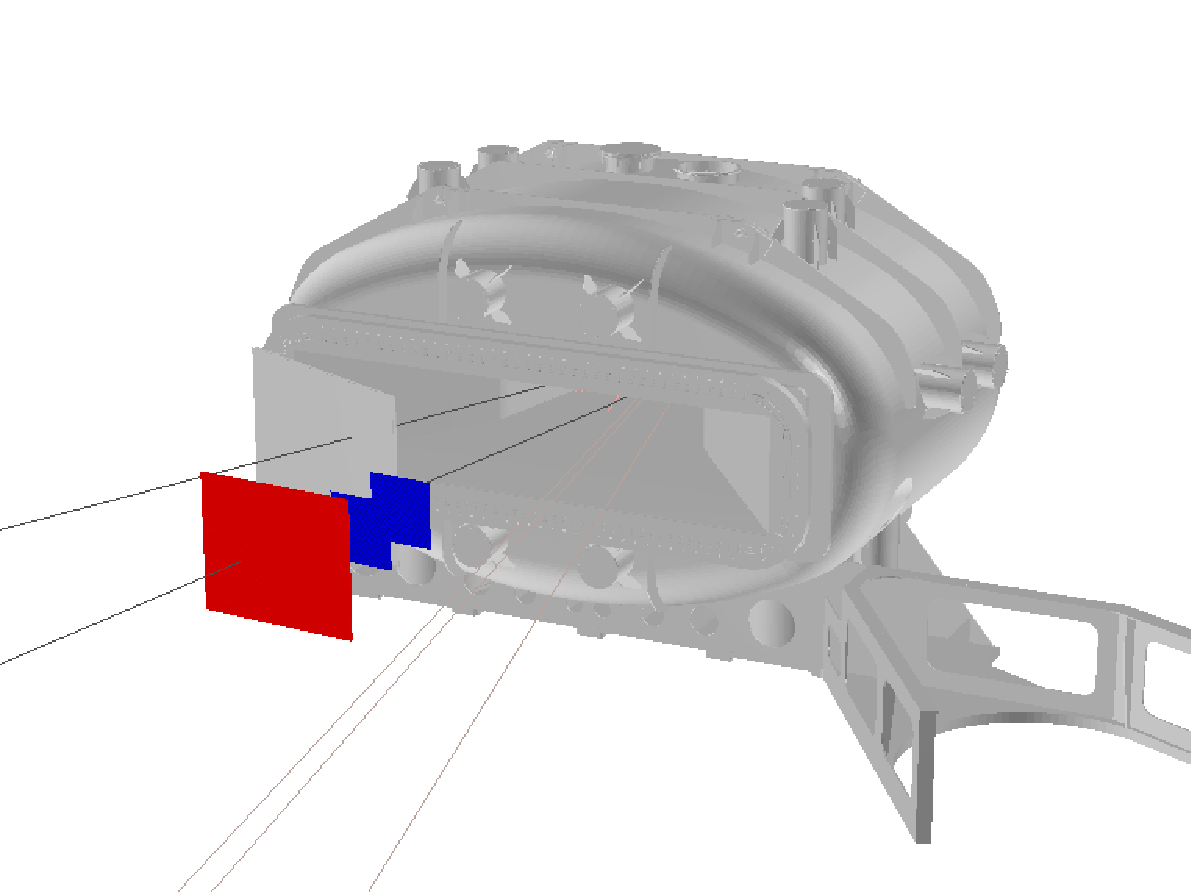
\includegraphics[width=0.6\linewidth]{/Simulations/SimEvEx}
	\caption[Example of a simulated event]{Example of an event in a simulation. In this case, there's a $^{14}$C passing through \gls{ToFD}, a Deuteron passing through the \gls{RPC} and 3 neutrons going to NeuLAND.}
	\label{fig:Simulation}
\end{figure}

%\section{Geant4}

%Geant4 \cite{agostinelli_geant4simulation_2003} is a C++ toolkit developed by CERN for simulating the passage of particles through matter. It provides detailed physics models and tracking capabilities that allow for realistic modeling of particle interactions, energy loss, multiple scattering, and nuclear processes. Within R3BRoot, Geant4 is responsible for handling the physical transport of particles through the simulated experimental setup, including interactions with detector materials, magnetic fields, and other components. This embedded use of Geant4 ensures that the simulations reflect the underlying physics of the experiment with high fidelity.


%\section{ROOT}

%ROOT \cite{brun_root_1997} is an object-oriented data analysis framework that provides tools for statistical analysis, histogramming, visualization, and data storage. R3BRoot integrates ROOT to manage event data, apply reconstruction algorithms, visualize results, and store output in ROOT-compatible formats. ROOT’s capabilities are essential for handling the large volumes of simulated data produced and for performing the subsequent analysis and validation steps.


%\section{R3BRoot}

%R3BRoot \cite{bertini_r3broot_2011} is the main framework used throughout this thesis for performing all simulation and analysis tasks. Developed specifically for experiments at the \gls{R3B} setup, R3BRoot builds on the FairRoot framework \cite{al-turany_fairroot_2012} and incorporates both Geant4 and ROOT. It provides pre-configured detector geometries, digitization routines, reconstruction algorithms, and analysis tools tailored to the \gls{R3B} experimental environment.

%Using R3BRoot, detailed simulations of the $^{25}$F(p,2p)$^{24}$O experiment were performed, including particle generation, tracking through the GLAD magnet, propagation through the tracking detectors and the \gls{RPC}, and emulation of detector responses. The framework also allowed the incorporation of realistic detector resolutions and systematics, enabling the generation of data that closely mirrors what will be observed experimentally. This simulated data also formed the basis for developing and validating the Multidimensional Fitting functions presented in this thesis.


\section{Simulation and Analysis Frameworks}

The simulations and analysis in this thesis were performed with \texttt{R3BRoot} \cite{bertini_r3broot_2011}, a framework specifically developed for the \gls{R3B} collaboration. It extends the FairRoot framework \cite{al-turany_fairroot_2012} and integrates two key tools in nuclear and high-energy physics: \texttt{Geant4} \cite{agostinelli_geant4simulation_2003} and \texttt{ROOT} \cite{brun_root_1997}.  

Within this environment, \texttt{Geant4} provides the physics engine for simulating the transport of particles through the experimental setup, accounting for interactions with detector materials, magnetic fields, and nuclear processes. This ensures that the modeled trajectories and energy losses accurately reflect the underlying physics.  

\texttt{ROOT} serves as the backbone for data handling and analysis. It enables efficient storage of simulated events, statistical analysis, and visualization, as well as the application of reconstruction algorithms to large datasets.  

By combining these elements, \texttt{R3BRoot} enables detailed end-to-end simulations of the $^{25}$F(p,2p)$^{24}$O experiment. Particle generation, transport through the GLAD magnet and tracking detectors, and detection in the RPC were modeled with realistic detector resolutions and systematics. The resulting datasets not only replicate expected experimental conditions but also formed the basis for training and validating the multidimensional fitting (MDF) functions presented later in this chapter.  
 


\section{Simulation of Expected Fragments at the RPC}

To evaluate the performance of the \gls{RPC} and anticipate the type of particles reaching it during the experiment, dedicated simulations were performed using the R3BRoot framework. These simulations aimed to estimate the expected fragment distribution at the \gls{RPC} detector and to assess the feasibility of studying additional physics channels beyond the primary reaction.

For this purpose, an INCL-generated event file corresponding to the reaction $^{22}$O + p was used as input. While this is not the main reaction under investigation ($^{25}$F(p,2p)$^{24}$O), its inclusion is highly relevant since $^{22}$O is predicted to be the dominant contaminant in the secondary beam, with an expected rate even higher than that of $^{25}$F, as seen in Figure \ref{fig:CocktailBeam}. Therefore, this simulation provides a realistic scenario for evaluating the \gls{RPC} response under experimental conditions.

The geometry used for this study assumed floating detector volumes, meaning that the physical structures and electronics of the detectors were not included in the simulation. This simplification was chosen to accelerate the computation and focus on the kinematics of the fragments.

The primary observable analyzed was the correlation between the atomic number (Z) and the mass-to-charge ratio (A/Z) of the fragments arriving at the \gls{RPC}, as shown in Figure \ref{fig:ZvsAoZ}. The results indicate that the most common fragments expected at the \gls{RPC} are deuterons and alpha particles, and that an A/Z ratio of 2, dominates the distribution. This information is essential for defining reconstruction strategies and particle identification methods.

\begin{figure}
	\centering
	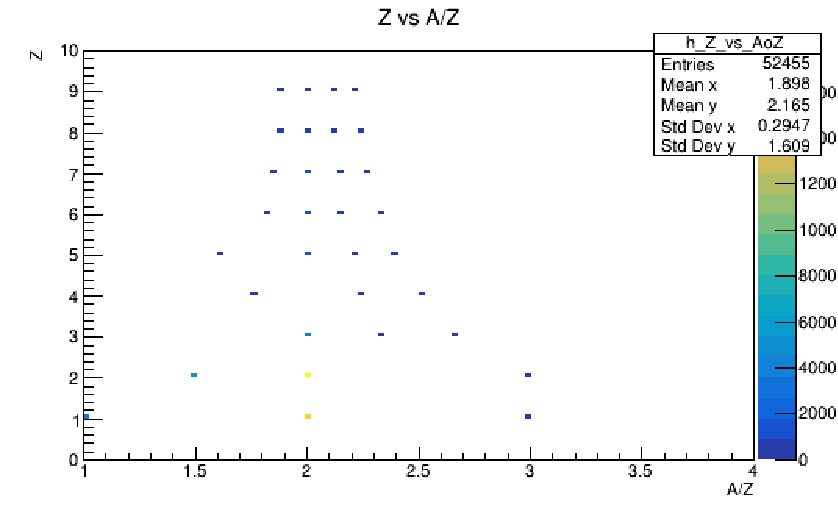
\includegraphics[width=0.8\linewidth]{/Simulations/ZvsAoZ}
	\caption[Fragment distribution reaching the RPC ($Z$ vs. $A/Z$)]{Distribution of fragments reaching the \gls{RPC}, shown as a correlation between the atomic number (Z) and the mass-to-charge ratio (A/Z). The most common fragments are deuterons and alpha particles, with A/Z = 2 being the dominant region.}
	\label{fig:ZvsAoZ}
\end{figure}

Furthermore, the simulation suggests that there may be opportunities to study additional reaction channels, such as (p,p$\alpha$), during the experimental campaign, provided that sufficient statistics are collected for these events.

A more detailed discussion of these simulations, including additional plots and distributions of fragment properties, is presented in Appendix \ref{app:rpc_plots}.

\section{Multidimensional Fitting}

In experiments like those conducted with the \gls{R3B} setup, the information directly recorded by detectors is often insufficient on its own to fully reconstruct the physical quantities of interest. Raw observables such as hit positions and times must be interpreted in the context of the particle’s full trajectory, charge, and energy. To bridge this gap, \gls{MDF} methods, a procedure of the ROOT framework \cite{ROOTMDF}, are used. These tools allow us to model complex, nonlinear relationships between measurable detector signals and the underlying physical properties of particles.

Multidimensional fitting is particularly powerful in the context of quasi-free scattering reactions, such as the one studied in the $^{25}$F(p,2p)$^{24}$O experiment. Given the diversity and overlap of signals produced by different particles and trajectories in the \gls{R3B} setup, \gls{MDF} enables a more accurate reconstruction of particle kinematics by using correlated detector data. It also allows us to compensate for the intrinsic limitations of individual detectors by combining information from multiple systems.

\subsection{Application to the RPC and FOOT Detectors}

In the simulation phase of this work, \gls{MDF} techniques were employed to enhance the reconstruction of particle kinematics at the \gls{RPC} detector — the main focus of this thesis. To train the fitting models, a realistic dataset was generated by simulating the propagation of particles expected to be detected in the experiment, namely protons, alpha particles, deuterons, and $^3$He nuclei. These particles were tracked from their production near the target, through the downstream tracking detectors (FOOTs), the GLAD magnet, and finally to the \gls{RPC}.

Eight input variables were selected to capture the relevant kinematic and spatial information of the particles:
\begin{enumerate}
	\item The x and y positions at the last pair of FOOT detectors;
	\item The directional angles of the particles (Tx and Ty), calculated from the positions at both pairs of FOOTs downstream of the target;
	\item The x, y and z positions at the \gls{RPC};
	\item The time of flight between the last FOOT and the \gls{RPC}.
\end{enumerate}


These features encapsulate the spatial evolution and timing of particles along their flight path, providing the necessary information to infer more abstract physical quantities.

A \gls{MDF} function to estimate the momentum over charge (p/Q) of particles was trained using this dataset.

Typically, in \gls{R3B} analyses, an additional \gls{MDF} function is trained to estimate the flight path of the particle. When combined with the reconstructed momentum-over-charge (p/Q), this allows the calculation of the particle’s velocity as a fraction of the speed of light ($\beta$) and the Lorentz factor ($\gamma$). These quantities are crucial for deriving the mass-to-charge ratio (A/Q), which plays an essential role in particle identification.

Initially, this approach was attempted in the present work by training a second \gls{MDF} to predict the flight path from the same set of observables. However, the fitting procedure for this \gls{MDF} did not converge properly and failed to provide a reliable minimization. This indicates that, given the chosen input variables, the correlation between the detector observables and the true flight path was not strong enough to allow for a robust fit.

To overcome this limitation, an alternative strategy was developed. Instead of estimating the flight path, a second \gls{MDF} function was trained to predict the mass-to-charge ratio (A/Q) directly. For this purpose, the original eight input variables were used, and an additional ninth variable was introduced: the value of p/Q obtained from the first \gls{MDF}. Including p/Q as an input significantly improved the predictive power of the second \gls{MDF}, enabling it to infer A/Q with high accuracy.

The performance of this new approach was evaluated using a dedicated validation process (see Section \ref{MDFValidation}), and the results were remarkably good. The differences between the predicted and true A/Q values were minimal, with uncertainties reaching the order of $10^{-3}$ in normalized units. This demonstrates that the method is not only viable but also highly precise, making it a strong candidate for application in real experimental data analysis.


These trained models can later be applied to experimental data to infer momentum and trajectory parameters with higher confidence than would be possible using analytic approximations alone.

This approach demonstrates the importance of data-driven tools like \gls{MDF} in modern nuclear physics experiments, where complexity and high dimensionality make traditional reconstruction methods insufficient.

\subsection{Validation of the MDF Models}
\label{MDFValidation}

Once the \gls{MDF} models were trained, their performance was validated using a new set of Geant4-based simulations that reproduced a realistic experimental scenario. These simulations included full beam-target reactions and accounted for detector resolution effects, ensuring that the generated observables reflected the uncertainties expected during actual data collection.

For each simulated event, the detector observables were extracted and used as input to the trained \gls{MDF} functions, which reconstructed the physical parameters of interest. These reconstructed values were then compared with the known "true" values from the Geant4 simulations. The comparison was performed through a series of performance plots, with particular emphasis on the correlation between Q and A/Q. By contrasting the distributions obtained directly from the simulation with those reconstructed by the \gls{MDF} functions, it was possible to visually and quantitatively assess the performance of the method (see Figures \ref{fig:QvsAoZ_true} and \ref{fig:QvsAoZ_mdf}).


\begin{figure}[ht]
	\centering
	
	\begin{subfigure}[b]{0.75\textwidth}
		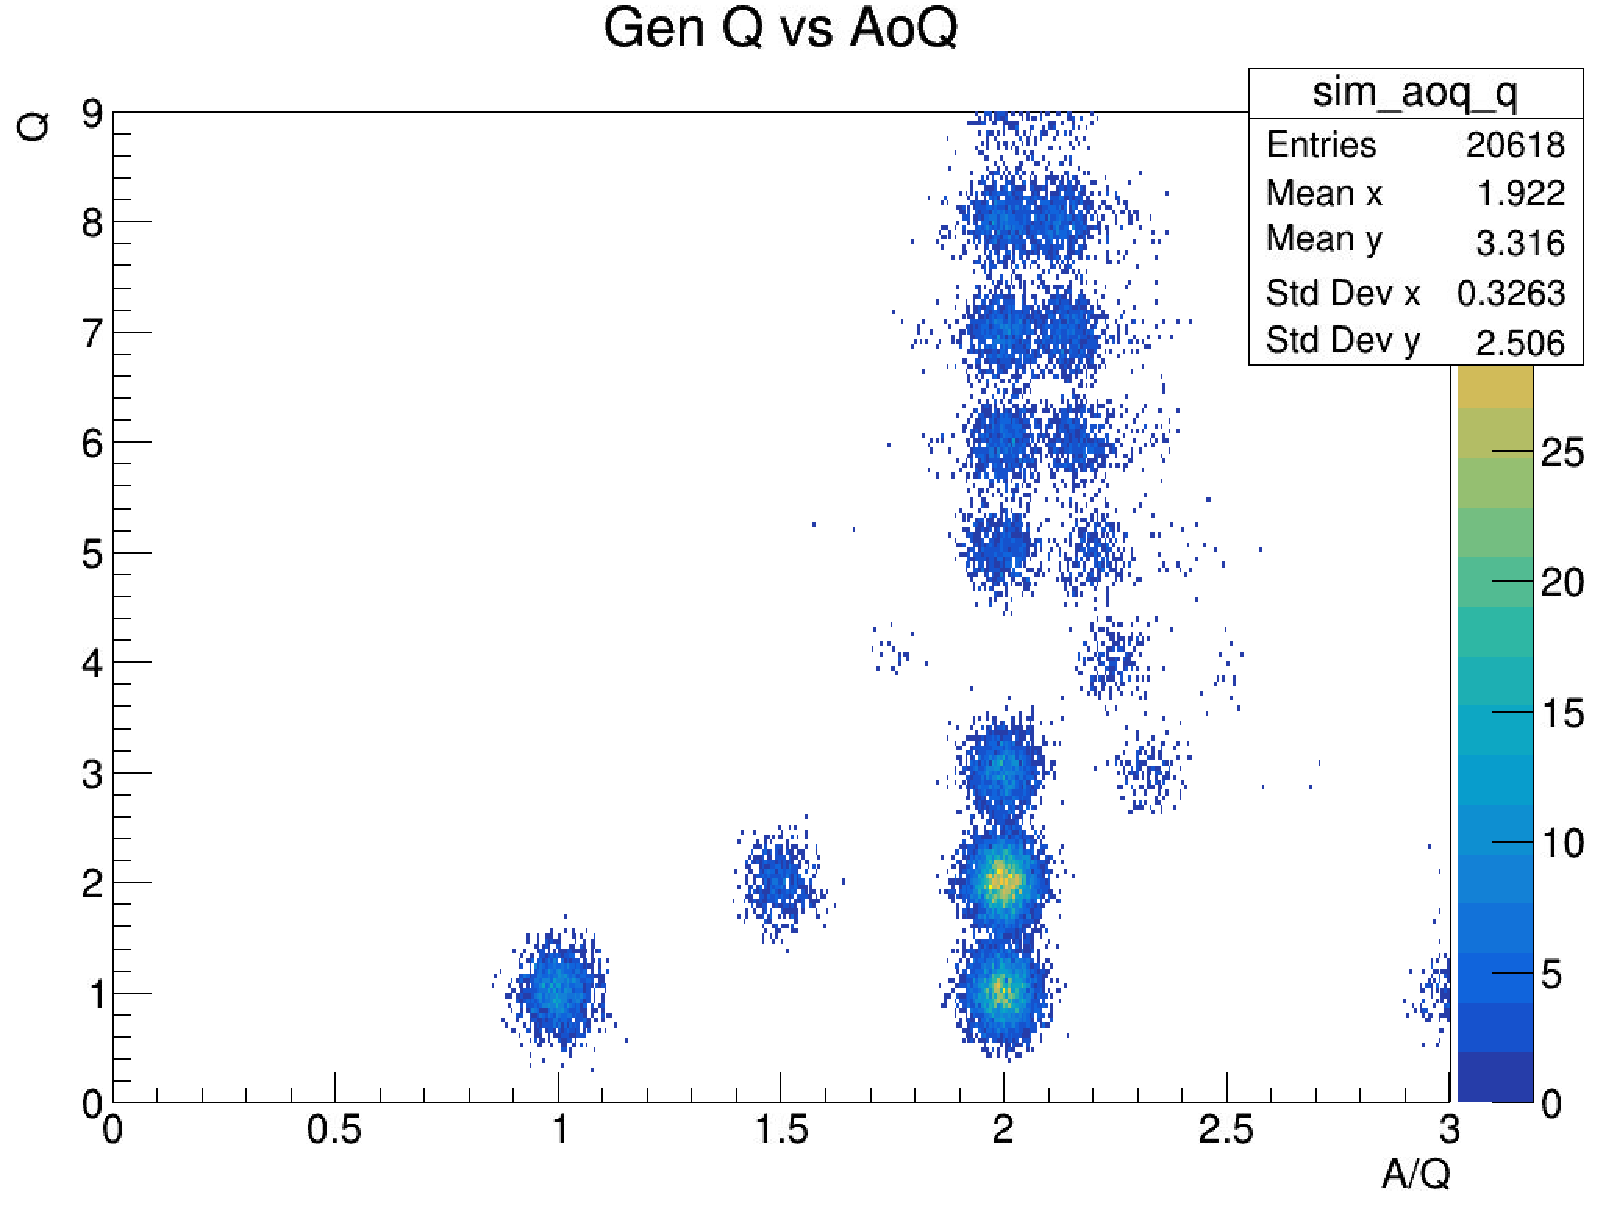
\includegraphics[width=1\linewidth]{/Simulations/QvsAoZ_true}
		\caption{Correlation between $Q$ and $A/Q$ obtained directly from Geant4 simulations, including detector resolution effects.}
		\label{fig:QvsAoZ_true} 
	\end{subfigure}
	
	\medskip % insert a bit of vertical whitespace
	\begin{subfigure}[b]{0.75\textwidth}
		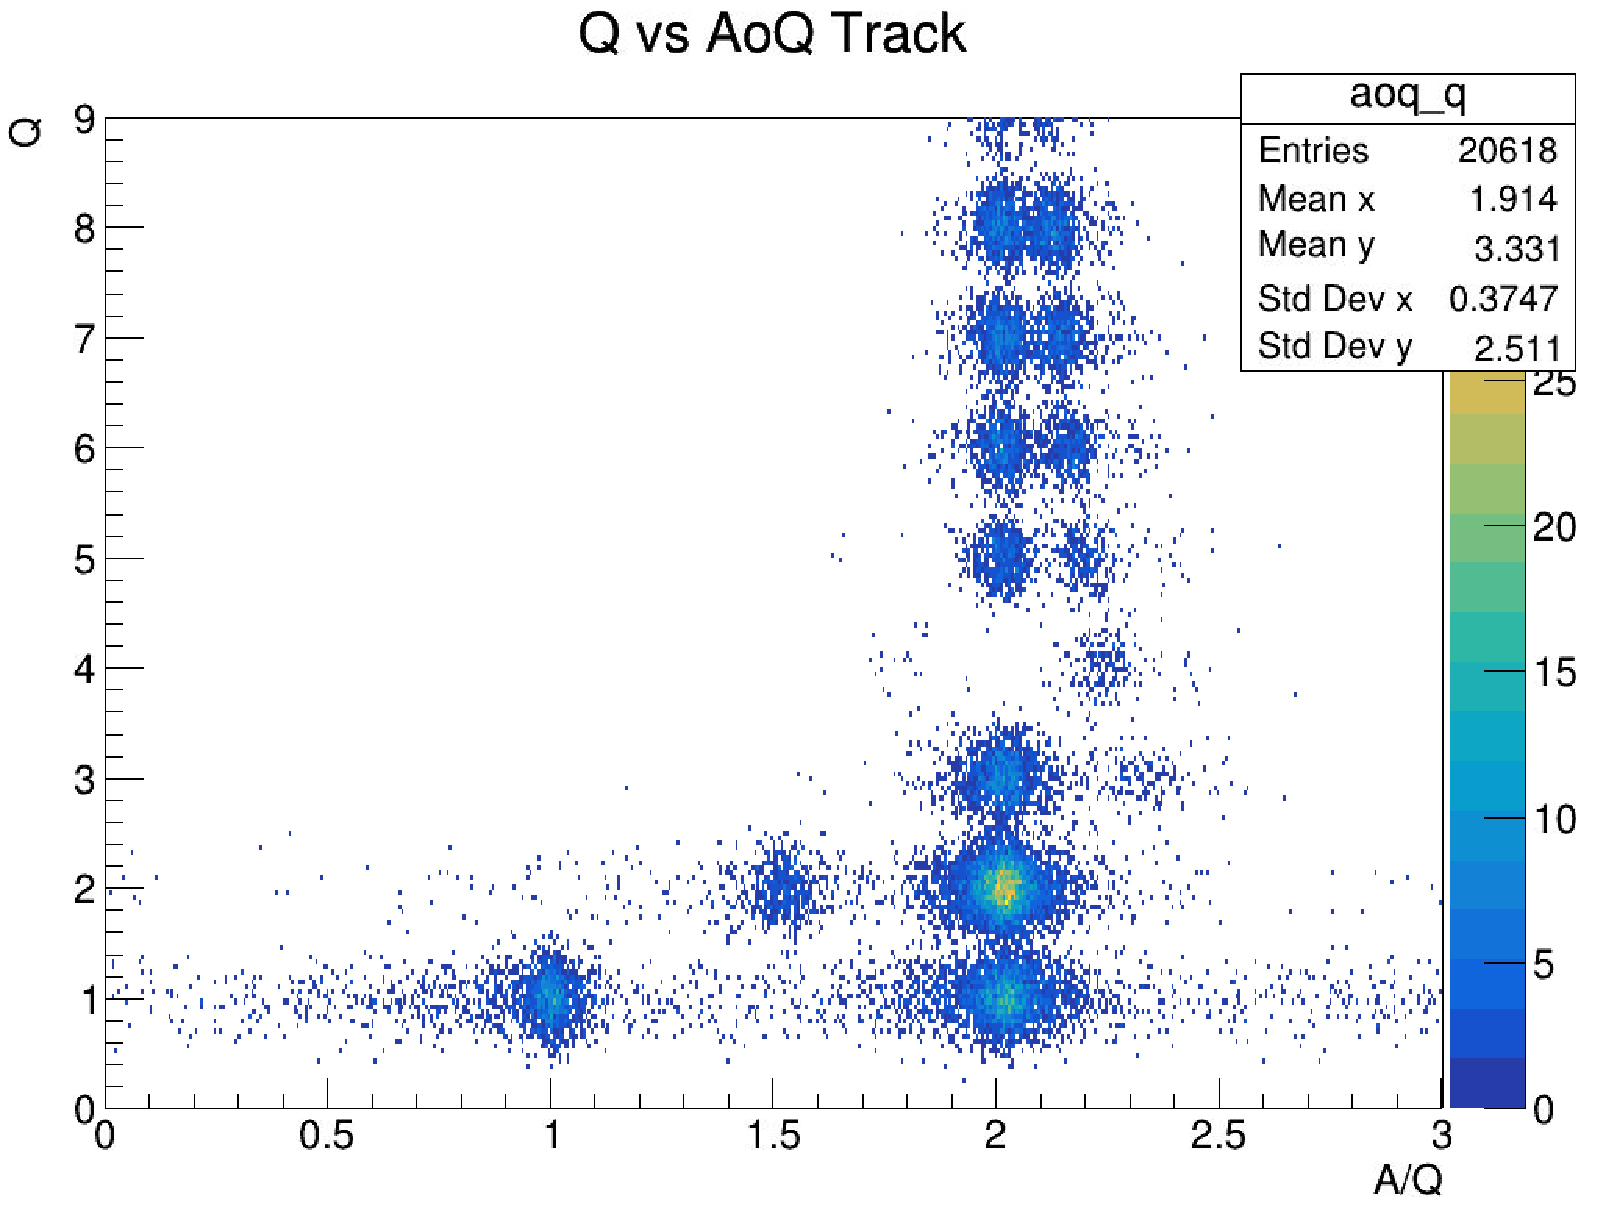
\includegraphics[width=1\linewidth]{/Simulations/QvsAoZ_mdf}
		\caption{Correlation between $Q$ and $A/Q$ reconstructed using the trained \gls{MDF} functions.}
		\label{fig:QvsAoZ_mdf}
	\end{subfigure}
	
	\caption[Comparison of simulated and reconstructed charge–mass correlations]{Comparison between simulated (a) and MDF-reconstructed (b) correlations of charge $Q$ and mass-to-charge ratio $A/Q$.}
	
\end{figure}

\section{Conclusions for the Experiment}

Based on the preliminary simulations with the INCL model, the main fragments expected to reach the \gls{RPC} are light ions, in particular deuterons and $\alpha$ particles. The results indicated that species with A/Q = 2 will dominate the detected distribution, reflecting the kinematic conditions and contaminant contributions from $^{22}$O. This outcome is relevant not only to anticipate the particle environment at the \gls{RPC}, but also to assess the feasibility of studying additional physics channels, such as (p,p$\alpha$) reactions.

The results of the \gls{MDF} method demonstrated excellent agreement between the reconstructed and simulated quantities. The residuals between predicted and true values were typically small, with uncertainties reaching down to the order of $10^{-3}$ in normalized units. This high level of precision confirms that the trained \gls{MDF} functions are robust and reliable under realistic conditions.

These findings are significant for the role of the \gls{RPC} detector within the \gls{R3B} setup. Traditionally, the \gls{RPC} has been considered primarily as a timing and proton detector, providing precise time-of-flight measurements for knocked out protons. However, the results of this study indicate that, in principle, the \gls{RPC} could also serve as a fragment reconstruction detector, provided that the \gls{MDF} method performs equally well when applied to real experimental data. This would increase the importance of the \gls{RPC} within the current experimental framework and could extend its potential role in future facilities, such as the \gls{FAIR} High Energy Cave, where enhanced fragment identification capabilities would be highly valuable.